\chapter{Introduction}
\par In Physiotherapy, tracking Range of Motion (ROM) is a standard approach to measuring progress in patient therapy. Often, ROM is measured subjectively and documentation is inconsistent between clinicians. Physios might come to wrong conclusions if ROM is tracked incorrectly between therapy sessions.

\begin{figure}[htbp]
	\centerline{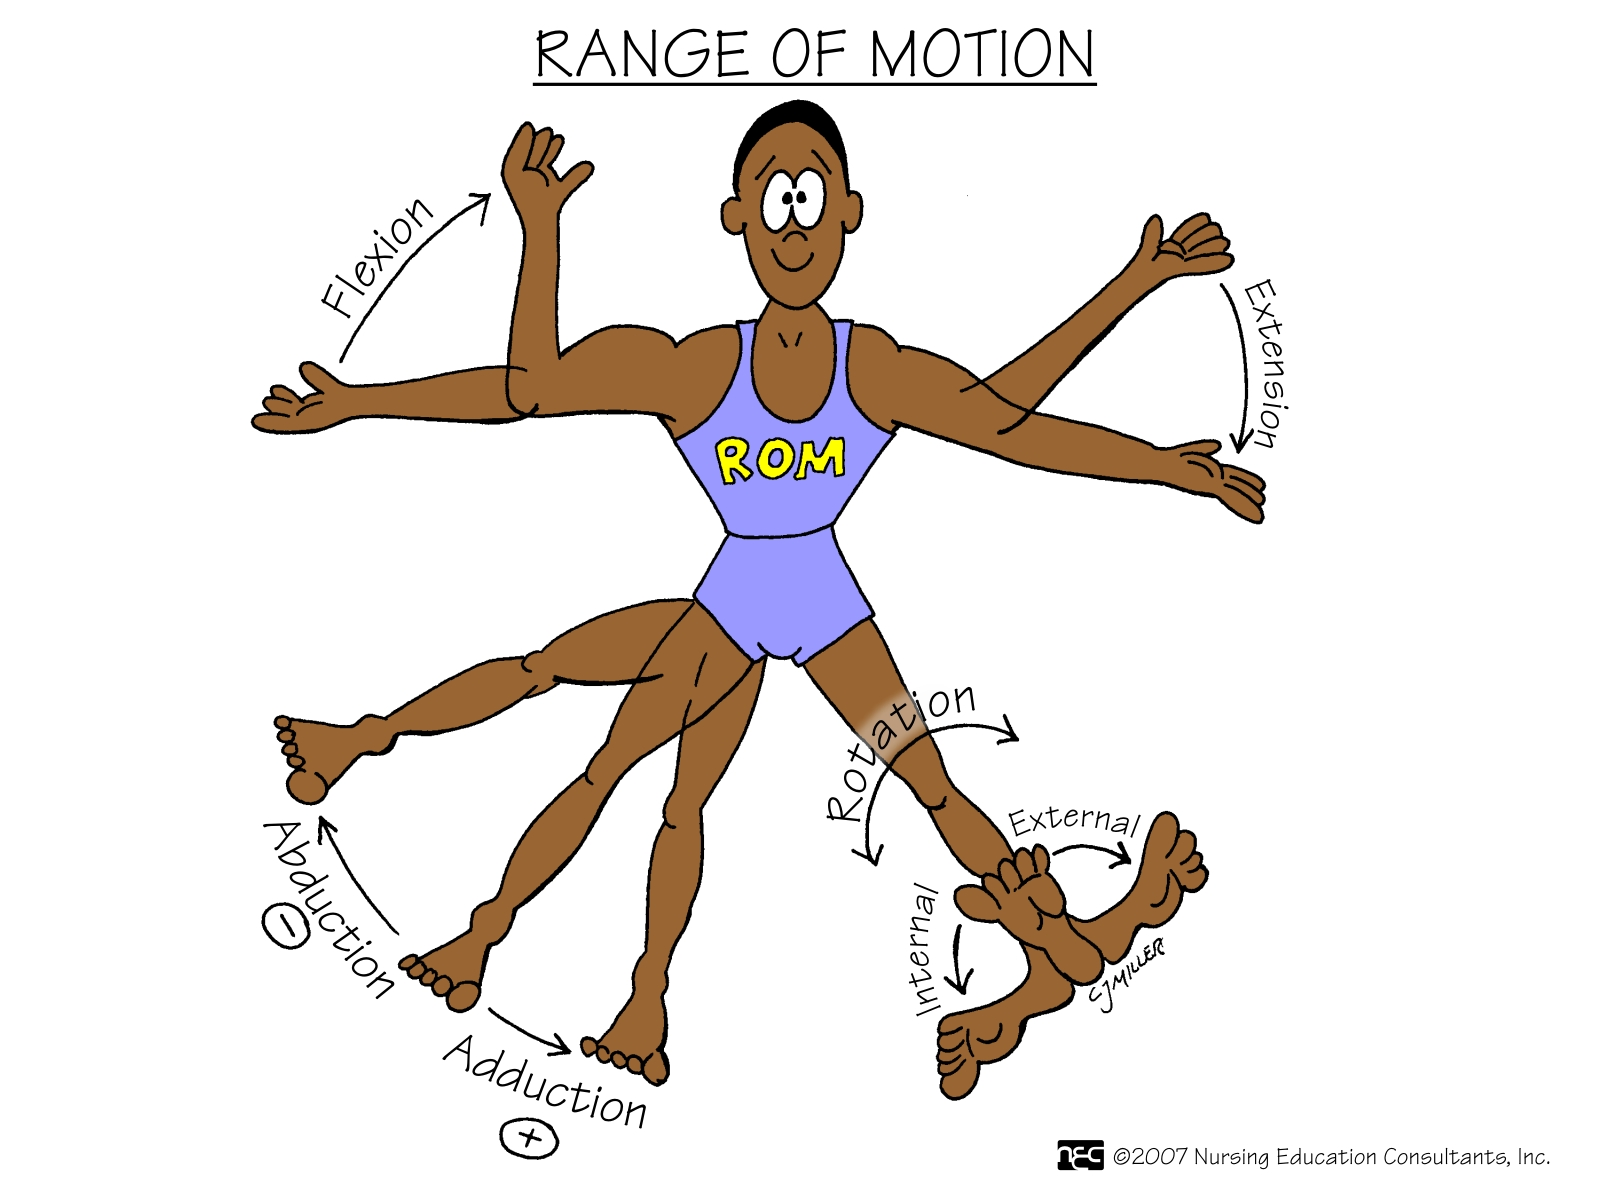
\includegraphics[scale=0.25]{fig/rangeofmotion.png}}  
	\caption{Range of Motion}
\end{figure}

\par The problem is that up to 70\% of patients give up physiotherapy because they can not see immediate results.
\par That's why we want to make a application which makes use of a phone camera to objectively calculate ROM in real-time and automatically produce a report that tracks progress over the course of several therapy sessions.

\section{Motivation}
\par Our motivation is to help patients who need physiotherapy to see a progress and to encourage them to be constant during their treatment. We want to support patients motivation in continuing to build new and healthy behaviours. 
\par This application is designed to help everyone who need physiotherapy treatment to stay motivated, reach their goals, and create habits that are healthy and helpful for a long term. In this case we have a solution by creating a app which will be a useful tool for patients who needs help to reach their goals by automated tracking of ROM.

\section{The purpose of the application}